This System Requirements Specification (SRS) describes the requirements for the \productname\ system. It is organized in accordance with the SRS information item defined in ISO/IEC/IEEE 29148:2018 \cite{ISO29148}, the current international standard for requirements engineering (which supersedes the withdrawn IEEE Std 830-1998). Replace this paragraph with a one-paragraph synopsis of the product and the purpose of this document.

\subsection{Purpose}
State the purpose of this SRS and identify the intended readership (customer, sponsor, team members, instructors, future maintainers). Explain that this document is the authoritative, agreed baseline of what the system shall do and shall not do, and that requirements in it may not be changed without agreement of the intended customer/sponsor.

\subsection{Scope}
Name the software/system product(s) to be produced. Explain what the product will and will not do, and describe the application and benefits of the product. Be careful to bound the scope: describe the boundary between this system and the external systems, users, and environment it interacts with.

\subsection{Product Overview}
Provide the context needed to understand the requirements that follow. Per ISO/IEC/IEEE 29148, address at least the four topics below.

\subsubsection{Product Perspective}
Describe how this product relates to other products or systems. Is it self-contained, a component of a larger system, or a replacement for an existing system? Include a high-level context diagram showing the system boundary, its users, and the external systems/interfaces it connects to.

\begin{figure}[h!]
	\centering
   	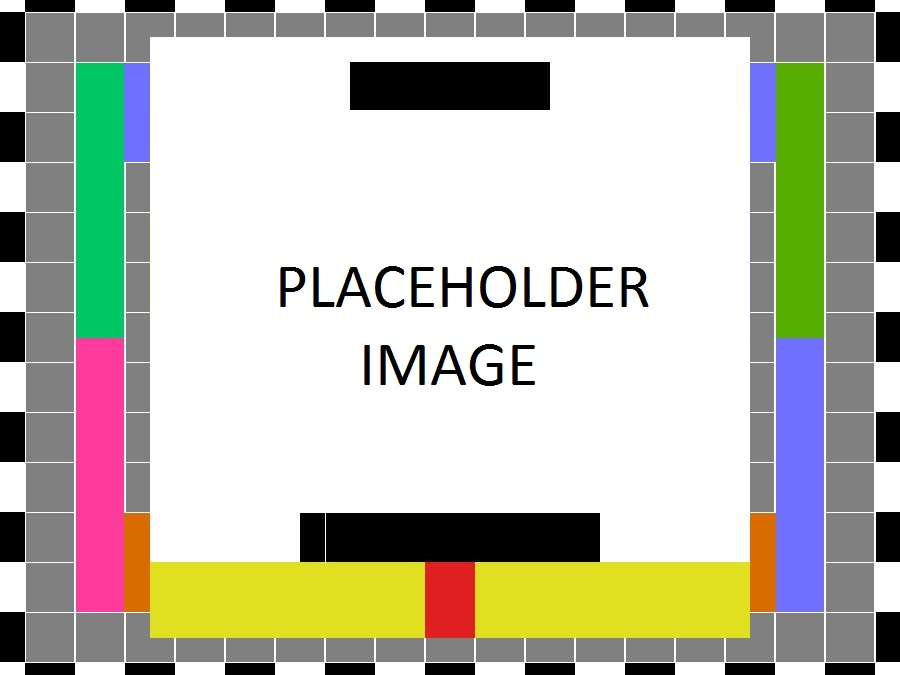
\includegraphics[width=0.60\textwidth]{images/test_image}
    \caption{\productname\ system context diagram}
\end{figure}

\subsubsection{Product Functions}
Summarize, at a high level, the major functions the product will perform. A bulleted list or a simple functional decomposition diagram is appropriate. Detailed, individually numbered requirements are specified in Sections 3--11; this subsection is only an orientation.

\subsubsection{User Characteristics}
Identify each class of user (end user, administrator, maintainer, external system) and the characteristics that affect requirements: expertise level, frequency of use, physical or accessibility considerations, and any assumptions about training.

\subsubsection{Assumptions \& Dependencies}
List the factors that, if changed, would change the requirements in this document. Distinguish assumptions (believed true but not guaranteed) from dependencies (relationships on external deliverables, systems, or organizations). Keep detailed project assumptions in the Project Charter; here, list only those that directly shape requirements.

\subsection{Definitions, Acronyms, and Abbreviations}
Define all terms, acronyms, and abbreviations required to interpret this document. A two-column table works well.

\begin{table}[H]
\caption{Definitions, acronyms, and abbreviations}
\begin{center}
    \begin{tabular}{ | p{3cm} | p{10cm} |}
    \hline
    \textbf{Term} & \textbf{Definition} \\ \hline
    SRS & System Requirements Specification \\ \hline
    Term & Definition of the term as used in this document \\ \hline
    \end{tabular}
\end{center}
\end{table}
